\documentclass[
11pt, % The default document font size, options: 10pt, 11pt, 12pt
%codirector, % Uncomment to add a codirector to the title page
]{charter} 




% El títulos de la memoria, se usa en la carátula y se puede usar el cualquier lugar del documento con el comando \ttitle
\titulo{Programador remoto de equipos electrónicos} 

% Nombre del posgrado, se usa en la carátula y se puede usar el cualquier lugar del documento con el comando \degreename
\posgrado{Carrera de Especialización en Sistemas Embebidos} 
%\posgrado{Carrera de Especialización en Internet de las Cosas} 
%\posgrado{Carrera de Especialización en Intelegencia Artificial}
%\posgrado{Maestría en Sistemas Embebidos} 
%\posgrado{Maestría en Internet de las cosas}

% Tu nombre, se puede usar el cualquier lugar del documento con el comando \authorname
\autor{Ing. José Mendoza} 

% El nombre del director y co-director, se puede usar el cualquier lugar del documento con el comando \supname y \cosupname y \pertesupname y \pertecosupname
\director{Mg. Ing. Sergio Starkloff}
\pertenenciaDirector{SURiX S.R.L} 
% FIXME:NO IMPLEMENTADO EL CODIRECTOR ni su pertenencia
\codirector{John Doe} % para que aparezca en la portada se debe descomentar la opción codirector en el documentclass
\pertenenciaCoDirector{FIUBA}

% Nombre del cliente, quien va a aprobar los resultados del proyecto, se puede usar con el comando \clientename y \empclientename
\cliente{Mg. Ing. Sergio Starkloff}
\empresaCliente{SURiX S.R.L}

% Nombre y pertenencia de los jurados, se pueden usar el cualquier lugar del documento con el comando \jurunoname, \jurdosname y \jurtresname y \perteunoname, \pertedosname y \pertetresname.
\juradoUno{Nombre y Apellido (1)}
\pertenenciaJurUno{pertenencia (1)} 
\juradoDos{Nombre y Apellido (2)}
\pertenenciaJurDos{pertenencia (2)}
\juradoTres{Nombre y Apellido (3)}
\pertenenciaJurTres{pertenencia (3)}
 
\fechaINICIO{22 de agosto de 2023}		%Fecha de inicio de la cursada de GdP \fechaInicioName
\fechaFINALPlan{10 de octubre de 2023} 	%Fecha de final de cursada de GdP
\fechaFINALTrabajo{10 de junio de 2024}	%Fecha de defensa pública del trabajo final


\begin{document}

\maketitle
\thispagestyle{empty}
\pagebreak


\thispagestyle{empty}
{\setlength{\parskip}{0pt}
\tableofcontents{}
}
\pagebreak


\section*{Registros de cambios}
\label{sec:registro}


\begin{table}[ht]
\label{tab:registro}
\centering
\begin{tabularx}{\linewidth}{@{}|c|X|c|@{}}
\hline
\rowcolor[HTML]{C0C0C0} 
Revisión & \multicolumn{1}{c|}{\cellcolor[HTML]{C0C0C0}Detalles de los cambios realizados} & Fecha      \\ \hline
v1.0      & Creación del documento                                 &\fechaInicioName \\ \hline
%1      & Se completa hasta el punto 4 inclusive                 & dd/mm/aaaa \\ \hline
v2.0      & Se completa hasta el punto 9 inclusive				& 28 de septiembre de 2023 \\ \hline
%		  Se puede agregar algo más \newline
%		  En distintas líneas \newline
%		  Así                                                    & dd/mm/aaaa \\ \hline
%3      & Se completa hasta el punto 11 inclusive                & dd/mm/aaaa \\ \hline
%4      & Se completa el plan	                                 & dd/mm/aaaa \\ \hline
\end{tabularx}
\end{table}

\pagebreak



\section*{Acta de constitución del proyecto}
\label{sec:acta}

\begin{flushright}
Buenos Aires, \fechaInicioName
\end{flushright}

\vspace{2cm}

Por medio de la presente se acuerda con el Ing. \authorname\hspace{1px} que su Trabajo Final de la \degreename\hspace{1px} se titulará ``\ttitle'', consistirá esencialmente en la implementación de un sistema que programe placas electrónicas mediante protocolo RS-232 y que los archivos de programación sean descargados por Wi-Fi y esos archivos podrán ser consultados a través de una página web, y tendrá un presupuesto preliminar estimado de 671 hs de trabajo, con fecha de inicio \fechaInicioName\hspace{1px} y fecha de presentación pública \fechaFinalName.

Se adjunta a esta acta la planificación inicial.

\vfill

% Esta parte se construye sola con la información que hayan cargado en el preámbulo del documento y no debe modificarla
\begin{table}[ht]
\centering
\begin{tabular}{ccc}
\begin{tabular}[c]{@{}c@{}}Dr. Ing. Ariel Lutenberg \\ Director posgrado FIUBA\end{tabular} & \hspace{2cm} & \begin{tabular}[c]{@{}c@{}}\clientename \\ \empclientename \end{tabular} \vspace{2.5cm} \\ 
\multicolumn{3}{c}{\begin{tabular}[c]{@{}c@{}} \supname \\ Director del Trabajo Final\end{tabular}} \vspace{2.5cm} \\
%\begin{tabular}[c]{@{}c@{}}\jurunoname \\ Jurado del Trabajo Final\end{tabular}     &  & \begin{tabular}[c]{@{}c@{}}\jurdosname\\ Jurado del Trabajo Final\end{tabular}  \vspace{2.5cm}  \\
%\multicolumn{3}{c}{\begin{tabular}[c]{@{}c@{}} \jurtresname\\ Jurado del Trabajo Final\end{tabular}} \vspace{.5cm}                                                                     
\end{tabular}
\end{table}




\section{1. Descripción técnica-conceptual del proyecto a realizar}
\label{sec:descripcion}


%\begin{consigna}{red} % El bloque "consigna" se usa para poner texto en rojo y dar una pequeña ayuda sobre cómo completar la sección. En cada entrega parcial deben eliminar los comandos begin y end del bloque consigna de las secciones que hayan completado.

El presente proyecto es realizado para la empresa SURiX. La empresa tiene un campo de actividad el cual es el desarrollo de productos que incluyan el protocolo IP, tales como portería, controles de acceso y anunciamientos.

La problemática actuál consiste en que la empresa tiene algunos productos (como controles de acceso) que solamente contemplan una interfaz de comunicación RS-232 para poder ser descargada una configuración.

La propuesta de proyecto consiste en diseñar un programador remoto que pueda cargar y descargar alguna configuración a un producto en específico mediante una interfaz de comunicación RS-232 y/o RS-285. Tal programador tendrá una conexión a internet mediante protocolo Wi-Fi para poder cargar y/o descargar los archivos de configuración. Estos archivos de configuración descargados por la placa conectada a internet serán descargados al control de acceso mediante una interfaz RS-232. De este modo se podrá actualizar los productos de SURiX de una forma remota. 

Además de los requerimientos anteriores, se diseñará una página web la cual interactuará con el servidor, enviándole comandos al programador remoto. Esta página web deberá ser capaz de cargar un archivo de configuración al servidor para que el programador remoto a diseñar pueda descargarlo o viceversa. Descargar un archivo de configuración que el programador remoto haya subido al servidor.
Por esto anterior se puede resumir el proyecto en unos puntos:

\begin{itemize}
	\item El proyecto es parte del programa de vinculación. Este proyecto será realizado para la empresa SURiX S.R.L.
	\item No existe algún tipo de financiamiento por parte de la empresa y tampoco hay un acuerdo de confidencialidad.
	\item El programador remoto a diseñar requiere de una conexión a internet mediante Wi-Fi o Ethernet.
	\item Se tendrá que diseñar una página web que servirá para almacenar el archivo de configuración el cual el programador remoto podrá descargar por Wi-Fi.
\end{itemize}



\begin{figure}[htpb]
\centering 
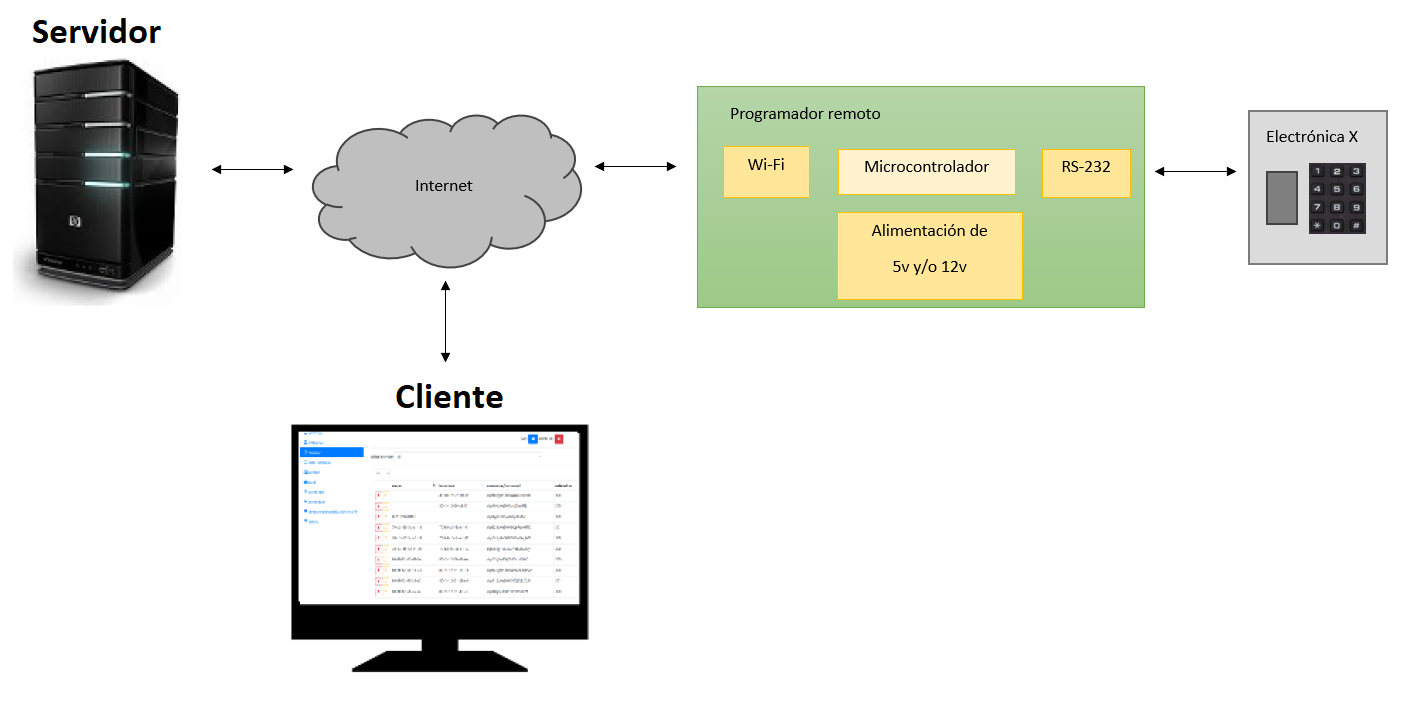
\includegraphics[width=1\textwidth]{./Figuras/DiagBloquesProgramador.png}
\caption{Diagrama en bloques del sistema}
\label{fig:diagBloques}
\end{figure}

\vspace{25px}

%\end{consigna}

\section{2. Identificación y análisis de los interesados}
\label{sec:interesados}


\begin{table}[ht]
%\caption{Identificación de los interesados}
%\label{tab:interesados}
\begin{tabularx}{\linewidth}{@{}|l|X|X|l|@{}}
\hline
\rowcolor[HTML]{C0C0C0} 
Rol           & Nombre y Apellido & Organización 	& Puesto 	\\ \hline
Cliente       & \clientename      &\empclientename	& Socio - Propietario \\ \hline
Responsable   & \authorname       & FIUBA        	& Alumno 	\\ \hline
Orientador    & \supname	      & \pertesupname 	& Director Trabajo final \\ \hline
Usuario final & Clientes de SURiX &       -      	&     -   	\\ \hline
\end{tabularx}
\end{table}



\begin{itemize}
	\item Cliente: Sergio Starkloff fue el que propuso el proyecto. Las reuniones con él son virtuales debido a que se encuentra fuera del país. En este proyecto también emplea el papel de Director.
	%\item Equipo: Juan Perez, suele pedir licencia porque tiene un familiar con una enfermedad. Planificar considerando esto.
	\item Orientador: Sergio Starkloff es también el orientador del proyecto. Cualquier duda técnica se le puede realizar a él.
	\item Usuario final: Los usuarios finales son los clientes de SURiX S.R.L que se ven en la necesidad de actualizar los productos de una forma remota.
\end{itemize}




\section{3. Propósito del proyecto}
\label{sec:proposito}


El propósito de este proyecto es desarrollar un programador remoto de equipos electrónicos . Este desarrollo permite poder cargar y descargar un archivo de configuracion a un servidor y además se desarrollará una página web en la que se podrá cargar los archivos de configuración que serán descargados al programador remoto.


\section{4. Alcance del proyecto}
\label{sec:alcance}

Para la realización del presente trabajo se incluyen las siguientes actividades:

\begin{itemize}
	\item Investigación y elección del hardware (microcontrolador) a utilizar.
	\item Diseño y desarrollo de página web para la carga y descarga de archivos de configuración.
	\item Investigación sobre comunicación FTP para la carga y descarga de archivos desde el servidor.
\end{itemize}

El presente proyecto no incluye:

\begin{itemize}
	\item Diseño de algún chasis que proteja físicamente la placa vinculada al proyecto.
	\item Algún diseño de circuito de protección de alimentación hacia la placa.
\end{itemize}


\section{5. Supuestos del proyecto}
\label{sec:supuestos}


Para el desarrollo del presente proyecto se supone que:

\begin{itemize}
	\item Se contará con una placa ESP32 para el desarrollo del proyecto.
	\item El tiempo de desarrollo del proyecto es ajustado a la duración de la especialidad.
	 \item Se diseñará una página web para la carga y descarga de archivos al servidor.
	 \item El cliente pondrá el servidor en el cual se almacenará la página web y los archivos de configuración.
	 \item Las pruebas del prototipo se realizarán en un servidor local ya el producto final estará en el servidor del cliente.
\end{itemize}


\section{6. Requerimientos}
\label{sec:requerimientos}

\begin{enumerate}
	\item Requerimientos generales de funcionamiento del sistema:
		\begin{enumerate}
			\item El sistema debe tener conexión a Wi-Fi.
			\item El sistema debe cargar y/o descargar un archivo de configuración desde un servidor.
			\item El sistema debe bajar el archivo de configuración a una tarjeta electrónica a través del protocolo de comunicación RS-232.
			\item El usuario debe poder cargar archivos de configuración al servidor desde una página web.
			\item La carga/descarga de archivos al servidor se realizará mediante protocol FTP.
			\item El sistema debe poder mandar una señal de reset a la tarjeta electrónica a programar.
		\end{enumerate}
	\item Requerimientos de la plataforma Web:
		\begin{enumerate}
			\item La plataforma Web debe permitir interactuar con el servidor para poder cargar y descargar archivos de configuración al y desde el servidor.
			\item La plataforma Web debe poder mandar comandos al sistema programador.
			
			
		\end{enumerate}
		
		
	\item Requerimientos del Firmware:
		\begin{enumerate}
			\item El firmware debe consultar periódicamente al servidor si hay algún comando a ejecutar.
			\item Deben existir al menos los siguientes comandos que el firmware debe interpretar:
			\begin{itemize}
				\item Configurar
				\item Descargar configuración
				\item Upload al servidor
				\item Download al servidor
				\item Reset
			\end{itemize}
		\end{enumerate}
	\item Requerimientos del Hardware:
		\begin{enumerate}
			\item El hardware debe de ser de bajo costo.
			\item Debe ser un microcontrolador popular en el mercado para que siempre exista disponibilidad de obtenerlo.
			\item Debe tener conexión a internet mediante Wi-Fi.
			\item Debe tener comunicación UART.
			\item Tener memoria flash para poder almacenar el archivo de configuración.
			\item Debe poder ser alimentado con 5V o 12V.
		\end{enumerate}
	\item Requerimientos de testing
		\begin{enumerate}
			\item Test unitario de cada función de software.
			\item Test de descarga de archivo del programador remoto hacia la placa a programar.
			\item Test de carga y descarga de archivo del programador remoto hacia el servidor.
			\item Test de carga y descarga de archivos hacia el servidor desde la plataforma Web.
			\item Test de envío de comandos desde la plataforma Web hacia el programador remoto.
		\end{enumerate}
	\item Requerimientos de documentación
		\begin{enumerate}
			\item El desarrollo estará acompañado de una memoria técnica.
			\item El desarrollo estará acompañado de una guía de usuario.
		\end{enumerate}
\end{enumerate}


\section{7. Historias de usuarios (\textit{Product backlog})}
\label{sec:backlog}

En el contexto actual la única historia de usuarios es la del cliente/director del proyecto, la cual sería la siguiente:
Se desea diseñar un programador remoto para poder actualizar diferentes productos como porteros y controles de acceso que cuenten con una interfaz RS-232, de forma remota, mandando comandos al programador por una página web. Una página web en lugar de una aplicación para pc sería mejor ya que no habría problemas de compatibilidad entre sistemas operativos para correr la aplicación.


\section{8. Entregables principales del proyecto}
\label{sec:entregables}

\begin{itemize}
	\item Prototipo del sistema
	\item Manual de usuario
	\item Código fuente del firmware
	\item Código fuente de la plataforma web
	\item Memorias del proyecto
\end{itemize}


\section{9. Desglose del trabajo en tareas}
\label{sec:wbs}

\begin{enumerate}
\item Planificación del proyecto
	\begin{enumerate}
	\item Definición de proyecto, alcances, requerimientos y plan de trabajo. (20 hs)
	\item Presentanción del proyecto. (20 hs)
	\end{enumerate}
\item Investigación y diseño del proyecto
	\begin{enumerate}
	\item Estudio de las familias de microcontroladores Espressif (10 hs)
	\item Análisis de periféricos necesarios para la aplicación (10 hs)
	\item Selección y compra de chip microcontrolador (10 hs)
	\end{enumerate}
\item Diseño de Hardware
	\begin{enumerate}
	\item Elaboración de diagrama esquemático para prototipo. (35 hs)
	\item Elaboración de PCB para pruebas. (35 hs)
	\end{enumerate}
\item Diseño de Firmware
	\begin{enumerate}
	\item Definición del diagrama de flujo del programa. (20 hs)
	\item Definición de máquina de estados del sistema. (20 hs)
	\item Desarrollo del código para la conexión UART. (30 hs)
	\item Desarrollo del código para la conexión a internet por medio de Wi-Fi. (40 hs)
	\item Desarrollo del código para la carga y descarga de archivos al servidor. (40 hs)
	\item Desarrollo del código para la transmisión de archivos del programador remoto a la placa electrónica a programar (40 hs).
	\end{enumerate}
\item Diseño de página web
	\begin{enumerate}
	\item Investigación de los lenguajes necesarios para el desarrollo de la página web. (18 hs)
	\item Diseño de mock-ups para la página web. (10 hs)
	\item Diseño de la página web. (40 hs)
	\end{enumerate}
\item Testing
	\begin{enumerate}
	\item Prueba de conexión del programador remoto con el servidor. (25 hs)
	\item Prueba de carga y descarga de archivos desde el programador remoto hacia el servidor mediante protocolo FTP. (25 hs)
	\item Prueba de la aplicación web. (30 hs)
	\item Prueba de mando de comandos desde la página web hacia el programador remoto. (33 hs)
	\item Prueba carga y descarga de archivos desde la página web hacia el servidor. (30 hs)
	\end{enumerate}
\item Documentación
	\begin{enumerate}
	\item Elaboración de manual de usuario. (35 hs)
	\item Elaboración de manual para el desarrollador. (30 hs)
	\end{enumerate}
\item Memorias y presentación final
	\begin{enumerate}
	\item Escritura de memoria técnica. (40 hs)
	\item Preparación de presentanción del trabajo final. (25 hs)
	\end{enumerate}
\end{enumerate}

Cantidad total de horas: 671 hs

\section{10. Diagrama de Activity On Node}
\label{sec:AoN}

\begin{consigna}{red}
Armar el AoN a partir del WBS definido en la etapa anterior. 

%La figura \ref{fig:AoN} fue elaborada con el paquete latex tikz y pueden consultar la siguiente referencia \textit{online}:

%\url{https://www.overleaf.com/learn/latex/LaTeX_Graphics_using_TikZ:_A_Tutorial_for_Beginners_(Part_3)\%E2\%80\%94Creating_Flowcharts}

\end{consigna}

\begin{figure}[htpb]
\centering 
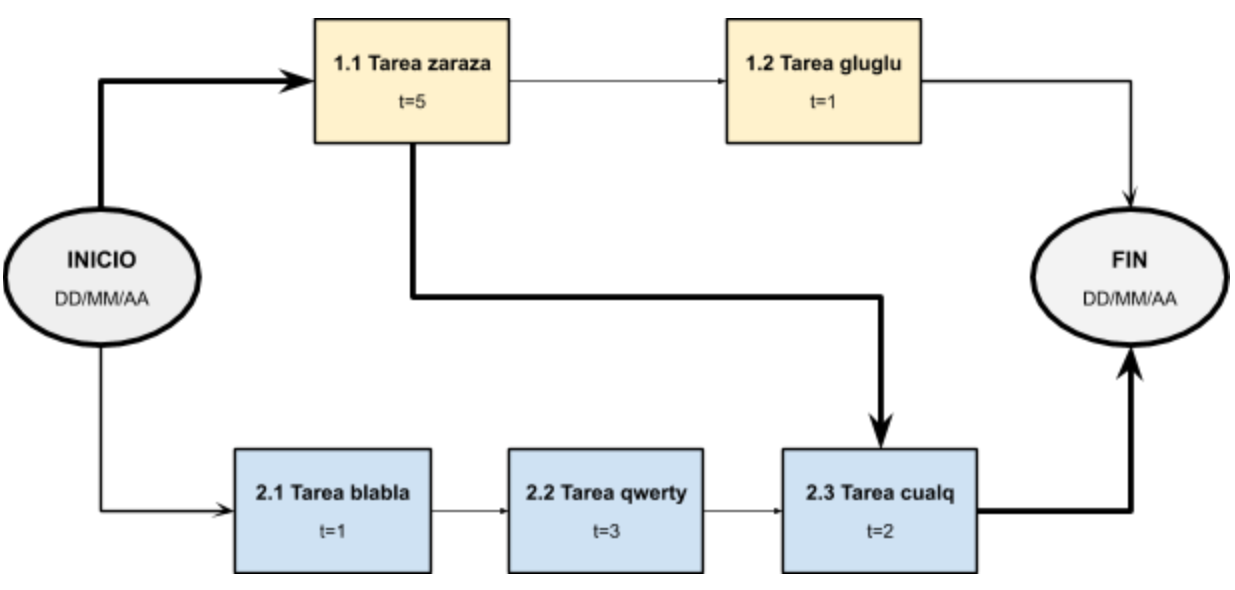
\includegraphics[width=.8\textwidth]{./Figuras/AoN.png}
\caption{Diagrama de \textit{Activity on Node}.}
\label{fig:AoN}
\end{figure}

Indicar claramente en qué unidades están expresados los tiempos.
De ser necesario indicar los caminos semicríticos y analizar sus tiempos mediante un cuadro.
Es recomendable usar colores y un cuadro indicativo describiendo qué representa cada color, como se muestra en el siguiente ejemplo:



\section{11. Diagrama de Gantt}
\label{sec:gantt}

\begin{consigna}{red}

Existen muchos programas y recursos \textit{online} para hacer diagramas de Gantt, entre los cuales destacamos:

\begin{itemize}
\item Planner
\item GanttProject
\item Trello + \textit{plugins}. En el siguiente link hay un tutorial oficial: \\ \url{https://blog.trello.com/es/diagrama-de-gantt-de-un-proyecto}
\item Creately, herramienta online colaborativa. \\\url{https://creately.com/diagram/example/ieb3p3ml/LaTeX}
\item Se puede hacer en latex con el paquete \textit{pgfgantt}\\ \url{http://ctan.dcc.uchile.cl/graphics/pgf/contrib/pgfgantt/pgfgantt.pdf}
\end{itemize}

Pegar acá una captura de pantalla del diagrama de Gantt, cuidando que la letra sea suficientemente grande como para ser legible. 
Si el diagrama queda demasiado ancho, se puede pegar primero la ``tabla'' del Gantt y luego pegar la parte del diagrama de barras del diagrama de Gantt.

Configurar el software para que en la parte de la tabla muestre los códigos del EDT (WBS).\\
Configurar el software para que al lado de cada barra muestre el nombre de cada tarea.\\
Revisar que la fecha de finalización coincida con lo indicado en el Acta Constitutiva.

En la figura \ref{fig:gantt}, se muestra un ejemplo de diagrama de Gantt realizado con el paquete de \textit{pgfgantt}. En la plantilla pueden ver el código que lo genera y usarlo de base para construir el propio.

\begin{figure}[htbp]
\begin{center}
\begin{ganttchart}{1}{12}
  \gantttitle{2020}{12} \\
  \gantttitlelist{1,...,12}{1} \\
  \ganttgroup{Group 1}{1}{7} \\
  \ganttbar{Task 1}{1}{2} \\
  \ganttlinkedbar{Task 2}{3}{7} \ganttnewline
  \ganttmilestone{Milestone o hito}{7} \ganttnewline
  \ganttbar{Final Task}{8}{12}
  \ganttlink{elem2}{elem3}
  \ganttlink{elem3}{elem4}
\end{ganttchart}
\end{center}
\caption{Diagrama de Gantt de ejemplo}
\label{fig:gantt}
\end{figure}


\begin{landscape}
\begin{figure}[htpb]
\centering 
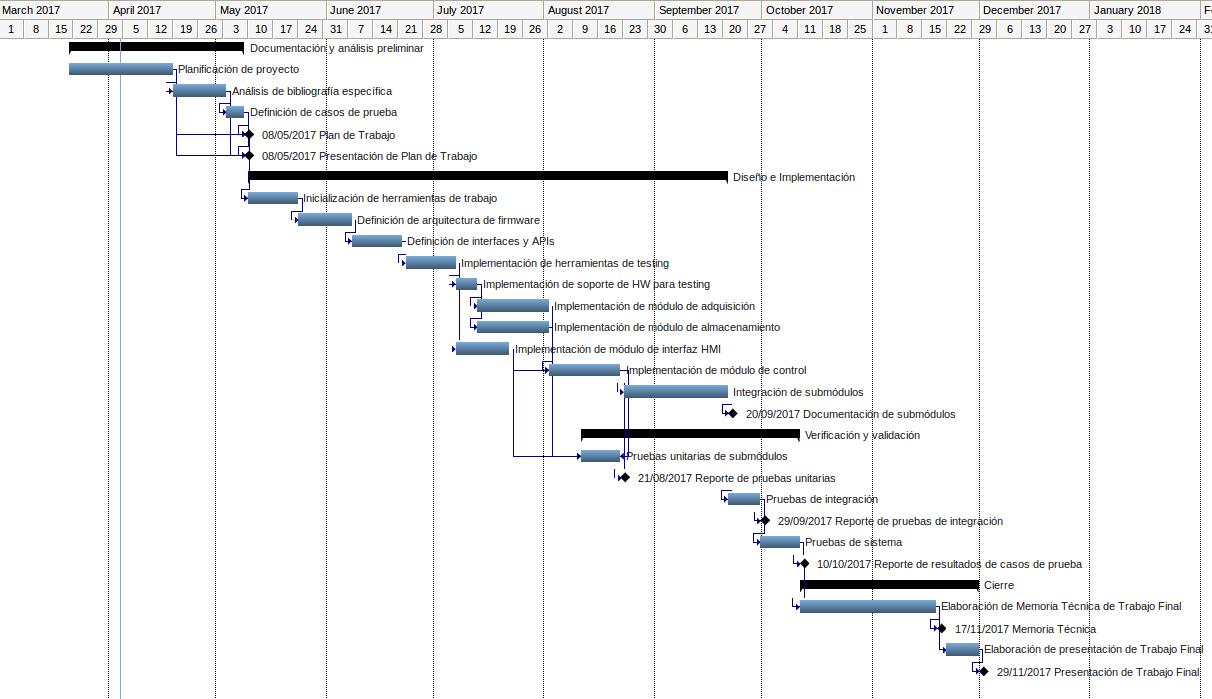
\includegraphics[height=.85\textheight]{./Figuras/Gantt-2.png}
\caption{Ejemplo de diagrama de Gantt rotado}
\label{fig:diagGantt}
\end{figure}

\end{landscape}

\end{consigna}


\section{12. Presupuesto detallado del proyecto}
\label{sec:presupuesto}

\begin{consigna}{red}
Si el proyecto es complejo entonces separarlo en partes:
\begin{itemize}
	\item Un total global, indicando el subtotal acumulado por cada una de las áreas.
	\item El desglose detallado del subtotal de cada una de las áreas.
\end{itemize}

IMPORTANTE: No olvidarse de considerar los COSTOS INDIRECTOS.

\end{consigna}

\begin{table}[htpb]
\centering
\begin{tabularx}{\linewidth}{@{}|X|c|r|r|@{}}
\hline
\rowcolor[HTML]{C0C0C0} 
\multicolumn{4}{|c|}{\cellcolor[HTML]{C0C0C0}COSTOS DIRECTOS} \\ \hline
\rowcolor[HTML]{C0C0C0} 
Descripción &
  \multicolumn{1}{c|}{\cellcolor[HTML]{C0C0C0}Cantidad} &
  \multicolumn{1}{c|}{\cellcolor[HTML]{C0C0C0}Valor unitario} &
  \multicolumn{1}{c|}{\cellcolor[HTML]{C0C0C0}Valor total} \\ \hline
 &
  \multicolumn{1}{c|}{} &
  \multicolumn{1}{c|}{} &
  \multicolumn{1}{c|}{} \\ \hline
 &
  \multicolumn{1}{c|}{} &
  \multicolumn{1}{c|}{} &
  \multicolumn{1}{c|}{} \\ \hline
\multicolumn{1}{|l|}{} &
   &
   &
   \\ \hline
\multicolumn{1}{|l|}{} &
   &
   &
   \\ \hline
\multicolumn{3}{|c|}{SUBTOTAL} &
  \multicolumn{1}{c|}{} \\ \hline
\rowcolor[HTML]{C0C0C0} 
\multicolumn{4}{|c|}{\cellcolor[HTML]{C0C0C0}COSTOS INDIRECTOS} \\ \hline
\rowcolor[HTML]{C0C0C0} 
Descripción &
  \multicolumn{1}{c|}{\cellcolor[HTML]{C0C0C0}Cantidad} &
  \multicolumn{1}{c|}{\cellcolor[HTML]{C0C0C0}Valor unitario} &
  \multicolumn{1}{c|}{\cellcolor[HTML]{C0C0C0}Valor total} \\ \hline
\multicolumn{1}{|l|}{} &
   &
   &
   \\ \hline
\multicolumn{1}{|l|}{} &
   &
   &
   \\ \hline
\multicolumn{1}{|l|}{} &
   &
   &
   \\ \hline
\multicolumn{3}{|c|}{SUBTOTAL} &
  \multicolumn{1}{c|}{} \\ \hline
\rowcolor[HTML]{C0C0C0}
\multicolumn{3}{|c|}{TOTAL} &
   \\ \hline
\end{tabularx}%
\end{table}


\section{13. Gestión de riesgos}
\label{sec:riesgos}

\begin{consigna}{red}
a) Identificación de los riesgos (al menos cinco) y estimación de sus consecuencias:
 
Riesgo 1: detallar el riesgo (riesgo es algo que si ocurre altera los planes previstos de forma negativa)
\begin{itemize}
	\item Severidad (S): mientras más severo, más alto es el número (usar números del 1 al 10).\\
	Justificar el motivo por el cual se asigna determinado número de severidad (S).
	\item Probabilidad de ocurrencia (O): mientras más probable, más alto es el número (usar del 1 al 10).\\
	Justificar el motivo por el cual se asigna determinado número de (O). 
\end{itemize}   

Riesgo 2:
\begin{itemize}
	\item Severidad (S): 
	\item Ocurrencia (O):
\end{itemize}

Riesgo 3:
\begin{itemize}
	\item Severidad (S): 
	\item Ocurrencia (O):
\end{itemize}


b) Tabla de gestión de riesgos:      (El RPN se calcula como RPN=SxO)

\begin{table}[htpb]
\centering
\begin{tabularx}{\linewidth}{@{}|X|c|c|c|c|c|c|@{}}
\hline
\rowcolor[HTML]{C0C0C0} 
Riesgo & S & O & RPN & S* & O* & RPN* \\ \hline
       &   &   &     &    &    &      \\ \hline
       &   &   &     &    &    &      \\ \hline
       &   &   &     &    &    &      \\ \hline
       &   &   &     &    &    &      \\ \hline
       &   &   &     &    &    &      \\ \hline
\end{tabularx}%
\end{table}

Criterio adoptado: 
Se tomarán medidas de mitigación en los riesgos cuyos números de RPN sean mayores a...

Nota: los valores marcados con (*) en la tabla corresponden luego de haber aplicado la mitigación.

c) Plan de mitigación de los riesgos que originalmente excedían el RPN máximo establecido:
 
Riesgo 1: plan de mitigación (si por el RPN fuera necesario elaborar un plan de mitigación).
  Nueva asignación de S y O, con su respectiva justificación:
  - Severidad (S): mientras más severo, más alto es el número (usar números del 1 al 10).
          Justificar el motivo por el cual se asigna determinado número de severidad (S).
  - Probabilidad de ocurrencia (O): mientras más probable, más alto es el número (usar del 1 al 10).
          Justificar el motivo por el cual se asigna determinado número de (O).

Riesgo 2: plan de mitigación (si por el RPN fuera necesario elaborar un plan de mitigación).
 
Riesgo 3: plan de mitigación (si por el RPN fuera necesario elaborar un plan de mitigación).

\end{consigna}


\section{14. Gestión de la calidad}
\label{sec:calidad}

\begin{consigna}{red}
Elija al menos diez requerientos que a su criterio sean los más importantes/críticos/que aportan más valor y para cada uno de ellos indique las acciones de verificación y validación que permitan asegurar su cumplimiento.

\begin{itemize} 
\item Req \#1: copiar acá el requerimiento.

\begin{itemize}
	\item Verificación para confirmar si se cumplió con lo requerido antes de mostrar el sistema al cliente. Detallar 
	\item Validación con el cliente para confirmar que está de acuerdo en que se cumplió con lo requerido. Detallar  
\end{itemize}

\end{itemize}

Tener en cuenta que en este contexto se pueden mencionar simulaciones, cálculos, revisión de hojas de datos, consulta con expertos, mediciones, etc.  Las acciones de verificación suelen considerar al entregable como ``caja blanca'', es decir se conoce en profundidad su funcionamiento interno.  En cambio, las acciones de validación suelen considerar al entregable como ``caja negra'', es decir, que no se conocen los detalles de su funcionamiento interno.

\end{consigna}

\section{15. Procesos de cierre}    
\label{sec:cierre}

\begin{consigna}{red}
Establecer las pautas de trabajo para realizar una reunión final de evaluación del proyecto, tal que contemple las siguientes actividades:

\begin{itemize}
	\item Pautas de trabajo que se seguirán para analizar si se respetó el Plan de Proyecto original:
	 - Indicar quién se ocupará de hacer esto y cuál será el procedimiento a aplicar. 
	\item Identificación de las técnicas y procedimientos útiles e inútiles que se emplearon, y los problemas que surgieron y cómo se solucionaron:
	 - Indicar quién se ocupará de hacer esto y cuál será el procedimiento para dejar registro.
	\item Indicar quién organizará el acto de agradecimiento a todos los interesados, y en especial al equipo de trabajo y colaboradores:
	  - Indicar esto y quién financiará los gastos correspondientes.
\end{itemize}

\end{consigna}


\end{document}
